\documentclass[a4paper, french]{article}
\usepackage{config}
\author{Vincent Commin \& Louis Leenart}
\date{\today}
\setcounter{secnumdepth}{6}
\begin{document}

\begin{titlepage}
    \begin{flushleft}
        
\includegraphics[width=5cm]{UL.jpg}\par
        \centering
        
        \vspace{13\baselineskip}       
        \HRule \\[0.4cm]

        {\Huge 
        GIF-4104 - TP 2\par}
        \vspace{0.4cm}
        \HRule
        \vfill
        Équipe 1 : Vincent Commin \& Louis Leenart\medskip \par
    \end{flushleft}
\end{titlepage}

\newpage
\section{Introduction}

Pour ce deuxième TP, nous avons du reprendre notre approche de parallélisation de recherche de
nombre premiers, en utilisant cette fois \textbf{OpenMP} au lieu de \textbf{pthread}. Nous utilisons
cependant encore une fois l'algorithme de
\href{https://fr.wikipedia.org/wiki/Test_de_primalit%C3%A9_de_Miller-Rabin}{\textit{\underline{Miller-Rabin}}}, et plus 
précisément l'implémentation de Stigen Larsen disponible sur
\href{https://github.com/cslarsen/miller-rabin}{\textit{\underline{Github}}}. Nous avons modifié
légèrement cette implémentation afin de permettre la parallélisation ainsi qu'améliorer les
performances. Enfin, notre algorithme supporte la recherche sur les grands notre, via la librairie
\href{https://gmplib.org/}{\textit{\underline{GMP}}}. \\\\\\

\section{Notre approche}

Dans ce TP, nous avons fait de notre mieux pour paralléliser notre algorithme en simplifiant un
maximum la lecture du code, tout en donnant des performances satisfaisantes. L'utilisation
d'OpenMP a permis de rendre le code beaucoup plus concis. L'algorithme que nous avons mis en place
est le suivant : 

\begin{lstlisting}[style=txt] 
premiers : vecteur de grands nombres 
intervalles : vecteur de pair de grands nombres
nb_threads : entier
tours : entier

// Section parallélisée sur nb_threads
POUR i ALLANT DE 0 A size(intervalles) FAIRE
    local_premiers : vecteur de grand nombres
    pair : pair de grands nombres = intervalles[i]
    aleatoire : générateur de nombre premier

    POUR j ALLANT DE pair.borne_basse A pair.borne_haute FAIRE
        est_premier : booléen = calculer_premier(j, tours, aleatoire)
        SI est_premier ALORS
            AJOUTER j DANS local_premiers
        FIN SI
    FIN POUR

    FUSIONNER local_premiers DANS premiers
FIN POUR
\end{lstlisting}

Aussi, afin de maximiser les performances, nous utilisons une fusion des intervalles pour limiter la
duplication des calculs. En effet, si deux intervalles se chevauchent, alors ils sont réunis en un
seul. Nous nous sommes inspirés de l'approche évoqué par l'équipe 3 dans leur rapport, et avons
implémenté notre propre algorithme adapté à notre structure de données. Nous avons rapidement
remarqué que la mise en place de cet algorithme a impacté grandement sur l'intérêt de la
parallélisation de certains fichiers. En effet, notre parallélisation consiste à répartir les
intervalles par threads, or la fusion d'intervalles a réduits certains fichiers à un seul interval. Nous
évoquerons cette difficulté plus en détails dans l'analyse. Aussi, l'algorithme utilisé pour la
fusion des intervalles est le suivant :

\newpage

\begin{lstlisting}[style=txt] 
intervalles : vecteur de pair de grands nombres
resultat : vecteur de pair de grands nombres

TRI intervalles SELON (a.premier < b.premier)

POUR pair : pair de grands nombres DANS intervalles FAIRE
    SI (resultat EST VIDE) OU (resultat.dernier.second < pair.second) ALORS
        AJOUTER pair A resultat
    SINON 
        resultat.dernier DEVIENT 
            (resultat.dernier.premier, 
            MAX(resultat.dernier.second, pair.second))
    FIN SI
FIN POUR
\end{lstlisting}

\section{Machine utilisée pour les tests de performance}

\begin{center}
    \begin{tabularx}{0.45\textwidth}{|>{\raggedleft\arraybackslash}X|>{\raggedright\arraybackslash}X|}
        \hline
        Modèle & intel i7-8550U \\
        \hline
        Architecture & x86\_64 \\
        \hline
        OS & Archlinux \\
        \hline
        Fréquence CPU & 3.4GHz \\
        \hline
        C\oe urs physiques & 4 \\
        \hline
        C\oe urs logiques & 8 \\
        \hline
        Ram & 16 Go, 2400 $MT/s$ \\
        \hline
    \end{tabularx}
\end{center}

\section{Résultats obtenus}

\begin{center}
    \begin{tabularx}{\textwidth}{c c}
        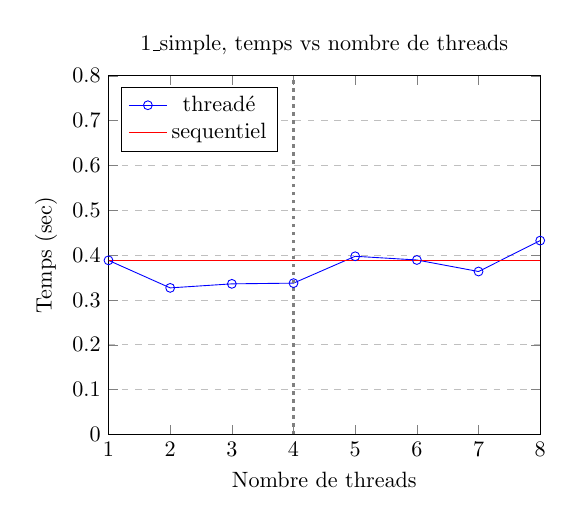
\begin{tikzpicture}[scale=0.8, transform shape]
            \begin{axis}[
                title={1\_simple, temps vs nombre de threads},
                xlabel={Nombre de threads},
                ylabel={Temps (sec)},
                xmin=1, xmax=8,
                ymin=0, ymax=0.8,
                xtick={1,2,3,4,5,6,7,8},
                ytick={0, 0.1, 0.2, 0.3, 0.4, 0.5, 0.6, 0.7, 0.8},
                legend pos=north west,
                ymajorgrids=true,
                grid style=dashed,
                ]        
                \addplot[color=blue, mark=o] coordinates {(1, 0.388412)(2, 0.327019)(3, 0.336002)(4, 0.337597)(5, 0.397522)(6, 0.389236)(7, 0.363555)(8, 0.432505)};   
                \addplot[color=red, mark=] coordinates {(1, 0.388412)(8, 0.388412)};
                \addplot[color=gray, dotted, ultra thick] coordinates {(4, 0)(4, 0.8)};
                \legend{threadé, sequentiel}
            \end{axis}
        \end{tikzpicture}
        & 
        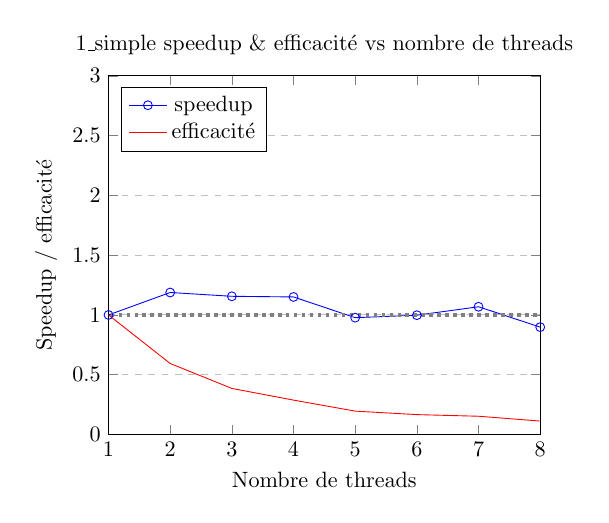
\begin{tikzpicture}[scale=0.8, transform shape]
            \begin{axis}[
                title={1\_simple speedup \& efficacité vs nombre de threads},
                xlabel={Nombre de threads},
                ylabel={Speedup / efficacité},
                xmin=1, xmax=8,
                ymin=0, ymax=3,
                xtick={1,2,3,4,5,6,7,8},
                ytick={0, 0.5, 1, 1.5, 2, 2.5, 3},
                legend pos=north west,
                ymajorgrids=true,
                grid style=dashed,
                ]        
                \addplot[color=blue, mark=o] coordinates {(1, 1)(2, 1.187735269)(3, 1.155981214)(4, 1.150519702)(5, 0.9770830294)(6, 0.9978830324)(7, 1.068372048)(8, 0.8980520456)};        
                \addplot[color=red, mark=] coordinates {(1, 1)(2, 0.5938676346)(3, 0.3853270715)(4, 0.2876299256)(5, 0.1954166059)(6, 0.1663138387)(7, 0.1526245783)(8, 0.112256505)};
                \addplot[color=gray, dotted, ultra thick] coordinates {(0, 1)(8, 1)};
                \legend{speedup, efficacité}
            \end{axis}
        \end{tikzpicture}
        \\
        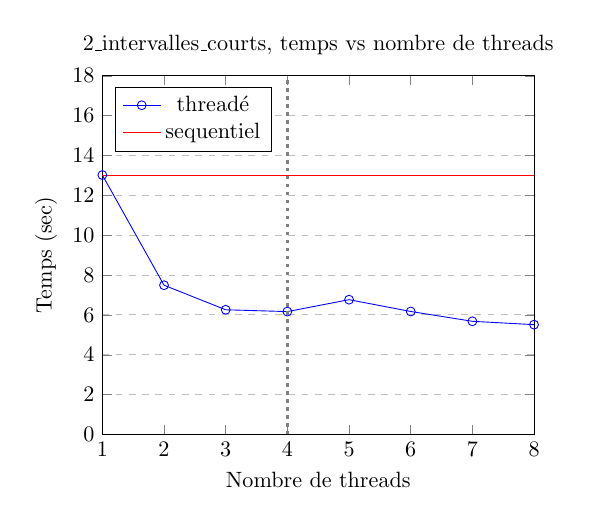
\begin{tikzpicture}[scale=0.8, transform shape]
            \begin{axis}[
                title={2\_intervalles\_courts, temps vs nombre de threads},
                xlabel={Nombre de threads},
                ylabel={Temps (sec)},
                xmin=1, xmax=8,
                ymin=0, ymax=18,
                xtick={1,2,3,4,5,6,7,8},
                ytick={0, 2, 4, 6, 8, 10, 12, 14, 16, 18},
                legend pos=north west,
                ymajorgrids=true,
                grid style=dashed,
                ]        
                \addplot[color=blue, mark=o] coordinates {(1, 13.0218)(2, 7.49222)(3, 6.25925)(4, 6.16795)(5, 6.76602)(6, 6.17349)(7, 5.68115)(8, 5.51193)};        
                \addplot[color=red, mark=] coordinates {(1, 13.0218)(8, 13.0218)};
                \addplot[color=gray, dotted, ultra thick] coordinates {(4, 0)(4, 18)};
                \legend{threadé, sequentiel}
            \end{axis}
        \end{tikzpicture}
        & 
        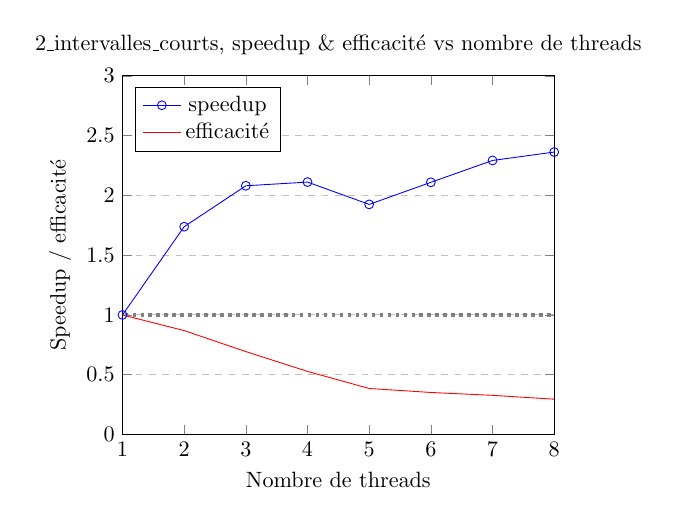
\begin{tikzpicture}[scale=0.8, transform shape]
            \begin{axis}[
                title={2\_intervalles\_courts, speedup \& efficacité vs nombre de threads},
                xlabel={Nombre de threads},
                ylabel={Speedup / efficacité},
                xmin=1, xmax=8,
                ymin=0, ymax=3,
                xtick={1,2,3,4,5,6,7,8},
                ytick={0, 0.5, 1, 1.5, 2, 2.5, 3},
                legend pos=north west,
                ymajorgrids=true,
                grid style=dashed,
                ]        
                \addplot[color=blue, mark=o] coordinates {(1, 1)(2, 1.73804293)(3, 2.080408995)(4, 2.111203885)(5, 1.924587867)(6, 2.109309321)(7, 2.292106352)(8, 2.362475576)};        
                \addplot[color=red, mark=] coordinates {(1, 1)(2, 0.8690214649)(3, 0.6934696649)(4, 0.5278009711)(5, 0.3849175734)(6, 0.3515515535)(7, 0.3274437645)(8, 0.295309447)};
                \addplot[color=gray, dotted, ultra thick] coordinates {(0, 1)(8, 1)};
                \legend{speedup, efficacité}
            \end{axis}
        \end{tikzpicture}
        \\ 
        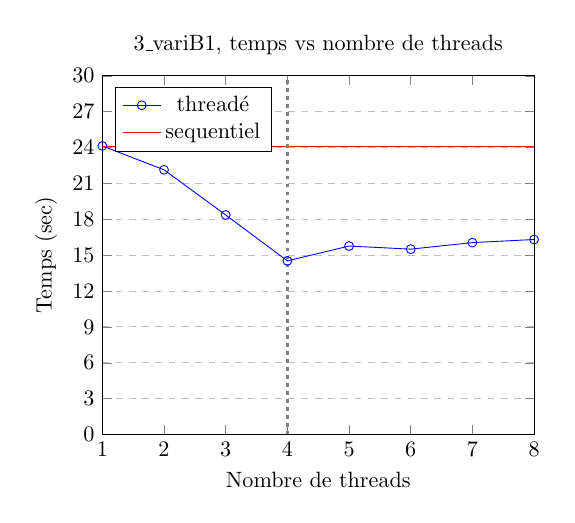
\begin{tikzpicture}[scale=0.8, transform shape]
            \begin{axis}[
                title={3\_variB1, temps vs nombre de threads},
                xlabel={Nombre de threads},
                ylabel={Temps (sec)},
                xmin=1, xmax=8,
                ymin=0, ymax=30,
                xtick={1,2,3,4,5,6,7,8},
                ytick={0, 3, 6, 9, 12, 15, 18, 21, 24, 27, 30},
                legend pos=north west,
                ymajorgrids=true,
                grid style=dashed,
                ]        
                \addplot[color=blue, mark=o] coordinates {(1, 24.1355)(2, 22.1384)(3, 18.3632)(4, 14.5218)(5, 15.7618)(6, 15.5036)(7, 16.0504)(8, 16.3093)};        
                \addplot[color=red, mark=] coordinates {(1, 24.1355)(8, 24.1355)};
                \addplot[color=gray, dotted, ultra thick] coordinates {(4, 0)(4, 30)};
                \legend{threadé, sequentiel}
            \end{axis}
        \end{tikzpicture}
        &
        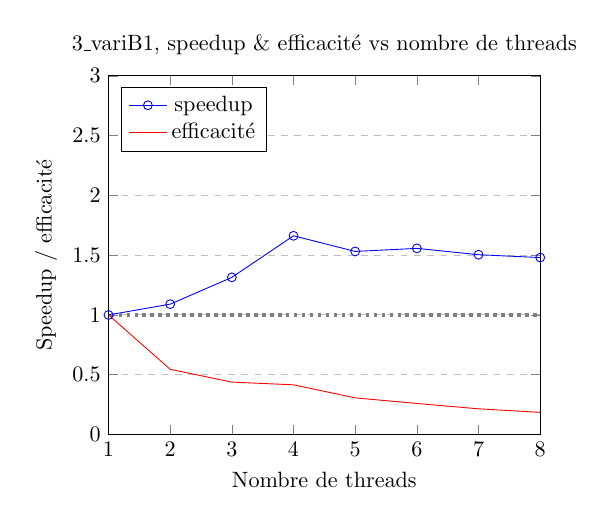
\begin{tikzpicture}[scale=0.8, transform shape]
            \begin{axis}[
                title={3\_variB1, speedup \& efficacité vs nombre de threads},
                xlabel={Nombre de threads},
                ylabel={Speedup / efficacité},
                xmin=1, xmax=8,
                ymin=0, ymax=3,
                xtick={1,2,3,4,5,6,7,8},
                ytick={0, 0.5, 1, 1.5, 2, 2.5, 3},
                legend pos=north west,
                ymajorgrids=true,
                grid style=dashed,
                ]        
                \addplot[color=blue, mark=o] coordinates {(1, 1)(2, 1.090209771)(3, 1.314340638)(4, 1.662018483)(5, 1.531265465)(6, 1.55676746)(7, 1.503731994)(8, 1.479861183)};        
                \addplot[color=red, mark=] coordinates {(1, 1)(2, 0.5451048856)(3, 0.4381135459)(4, 0.4155046206)(5, 0.3062530929)(6, 0.2594612434)(7, 0.2148188563)(8, 0.1849826479)};
                \addplot[color=gray, dotted, ultra thick] coordinates {(0, 1)(8, 1)};
                \legend{speedup, efficacité}
            \end{axis}
        \end{tikzpicture}
    \end{tabularx}
\end{center}

\newpage

\begin{center}
    \begin{tabularx}{\textwidth}{c c}
        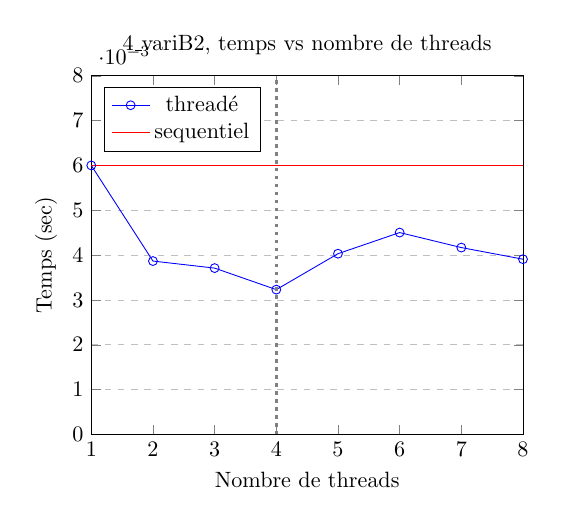
\begin{tikzpicture}[scale=0.8, transform shape]
            \begin{axis}[
                title={4\_variB2, temps vs nombre de threads},
                xlabel={Nombre de threads},
                ylabel={Temps (sec)},
                xmin=1, xmax=8,
                ymin=0, ymax=0.008,
                xtick={1,2,3,4,5,6,7,8},
                ytick={0, 0.001, 0.002, 0.003, 0.004, 0.005, 0.006, 0.007, 0.008},
                legend pos=north west,
                ymajorgrids=true,
                grid style=dashed,
                ]        
                \addplot[color=blue, mark=o] coordinates {(1, 0.00600104)(2, 0.00386856)(3, 0.00371145)(4, 0.00323145)(5, 0.0040326)(6, 0.00450418)(7, 0.00416944)(8, 0.00391003)};        
                \addplot[color=red, mark=] coordinates {(1, 0.00600104)(8, 0.00600104)};
                \addplot[color=gray, dotted, ultra thick] coordinates {(4, 0)(4, 0.008)};
                \legend{threadé, sequentiel}
            \end{axis}
        \end{tikzpicture}
        &
        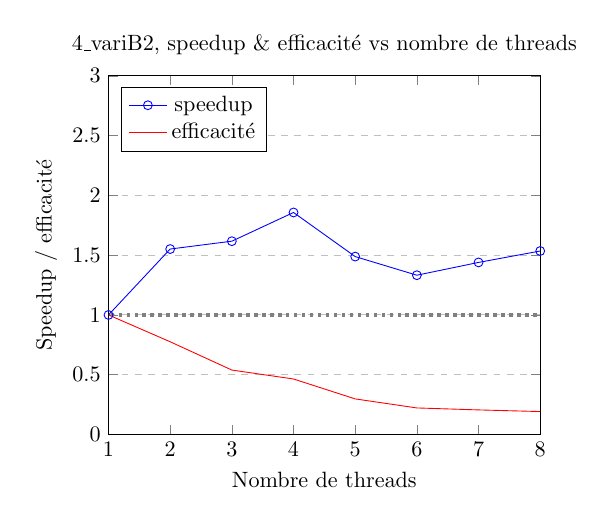
\begin{tikzpicture}[scale=0.8, transform shape]
            \begin{axis}[
                title={4\_variB2, speedup \& efficacité vs nombre de threads},
                xlabel={Nombre de threads},
                ylabel={Speedup / efficacité},
                xmin=1, xmax=8,
                ymin=0, ymax=3,
                xtick={1,2,3,4,5,6,7,8},
                ytick={0, 0.5, 1, 1.5, 2, 2.5, 3},
                legend pos=north west,
                ymajorgrids=true,
                grid style=dashed,
                ]        
                \addplot[color=blue, mark=o] coordinates {(1, 1)(2, 1.551233534)(3, 1.616899056)(4, 1.85707345)(5, 1.488131726)(6, 1.332326861)(7, 1.439291608)(8, 1.534781063)};        
                \addplot[color=red, mark=] coordinates {(1, 1)(2, 0.775616767)(3, 0.5389663519)(4, 0.4642683625)(5, 0.2976263453)(6, 0.2220544768)(7, 0.2056130868)(8, 0.1918476329)};
                \addplot[color=gray, dotted, ultra thick] coordinates {(0, 1)(8, 1)};
                \legend{speedup, efficacité}
            \end{axis}
        \end{tikzpicture}
        \\
        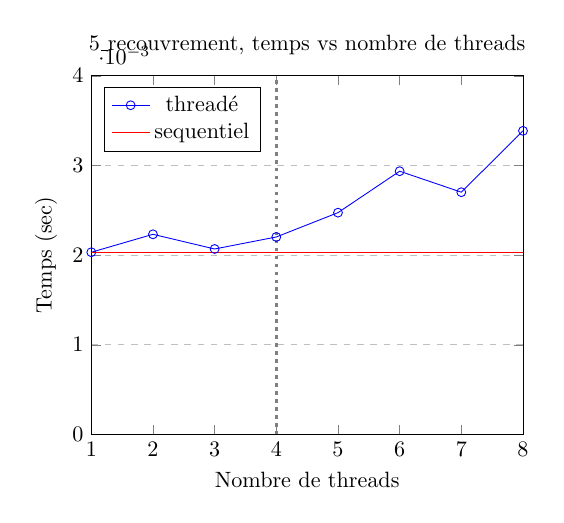
\begin{tikzpicture}[scale=0.8, transform shape]
            \begin{axis}[
                title={5\_recouvrement, temps vs nombre de threads},
                xlabel={Nombre de threads},
                ylabel={Temps (sec)},
                xmin=1, xmax=8,
                ymin=0, ymax=0.004,
                xtick={1,2,3,4,5,6,7,8},
                ytick={0, 0.001, 0.002, 0.003, 0.004},
                legend pos=north west,
                ymajorgrids=true,
                grid style=dashed,
                ]        
                \addplot[color=blue, mark=o]
                coordinates {(1, 0.00203256)(2, 0.00223267)(3, 0.00206891)(4, 0.00220282)(5, 0.00247404)(6, 0.00293645)(7, 0.00270223)(8, 0.00338652)};        
                \addplot[color=red, mark=] coordinates {(1, 0.00203256)(8, 0.00203256)};
                \addplot[color=gray, dotted, ultra thick] coordinates {(4, 0)(4, 0.004)};
                \legend{threadé, sequentiel}
            \end{axis}
        \end{tikzpicture}
        &
        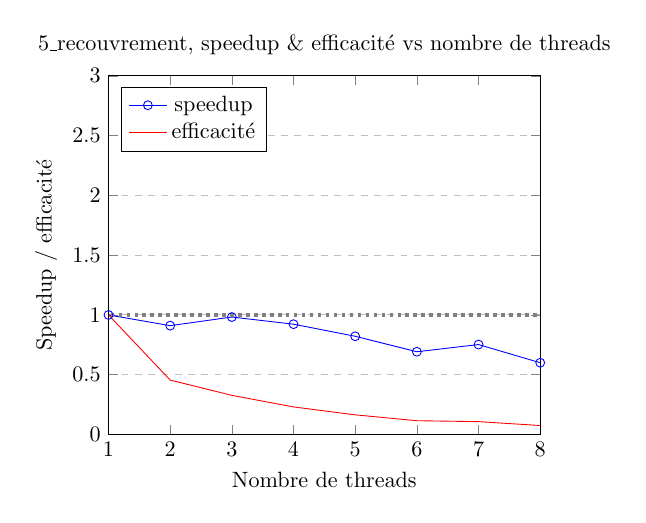
\begin{tikzpicture}[scale=0.8, transform shape]
            \begin{axis}[
                title={5\_recouvrement, speedup \& efficacité vs nombre de threads},
                xlabel={Nombre de threads},
                ylabel={Speedup / efficacité},
                xmin=1, xmax=8,
                ymin=0, ymax=3,
                xtick={1,2,3,4,5,6,7,8},
                ytick={0, 0.5, 1, 1.5, 2, 2.5, 3},
                legend pos=north west,
                ymajorgrids=true,
                grid style=dashed,
                ]        
                \addplot[color=blue, mark=o] coordinates {(1, 1)(2, 0.9103718866)(3, 0.9824303619)(4, 0.922708165)(5, 0.8215550274)(6, 0.6921827377)(7, 0.7521787561)(8, 0.6001913469)};        
                \addplot[color=red, mark=] coordinates {(1, 1)(2, 0.4551859433)(3, 0.3274767873)(4, 0.2306770412)(5, 0.1643110055)(6, 0.1153637896)(7, 0.107454108)(8, 0.07502391836)};
                \addplot[color=gray, dotted, ultra thick] coordinates {(0, 1)(8, 1)};
                \legend{speedup, efficacité}
            \end{axis}
        \end{tikzpicture}
        \\
        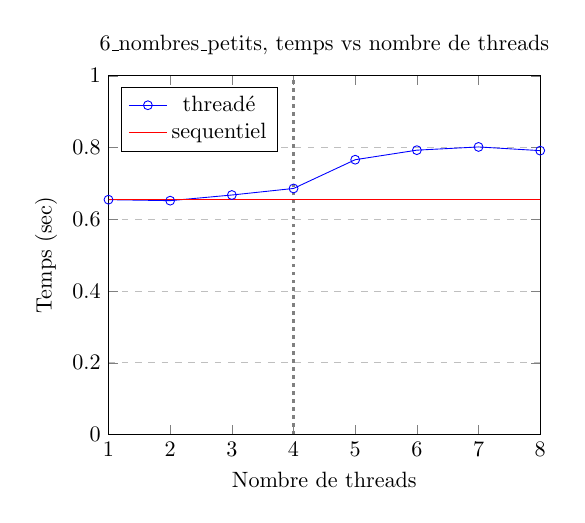
\begin{tikzpicture}[scale=0.8, transform shape]
            \begin{axis}[
                title={6\_nombres\_petits, temps vs nombre de threads},
                xlabel={Nombre de threads},
                ylabel={Temps (sec)},
                xmin=1, xmax=8,
                ymin=0, ymax=1,
                xtick={1,2,3,4,5,6,7,8},
                ytick={0, 0.2, 0.4, 0.6, 0.8, 1},
                legend pos=north west,
                ymajorgrids=true,
                grid style=dashed,
                ]        
                \addplot[color=blue, mark=o] coordinates {(1, 0.654738)(2, 0.651952)(3, 0.667715)(4, 0.685957)(5, 0.766144)(6, 0.792763)(7, 0.801771)(8, 0.791428)};        
                \addplot[color=red, mark=] coordinates {(1, 0.654738)(8, 0.654738)};
                \addplot[color=gray, dotted, ultra thick] coordinates {(4, 0)(4, 1)};
                \legend{threadé, sequentiel}
            \end{axis}
        \end{tikzpicture}
        &
        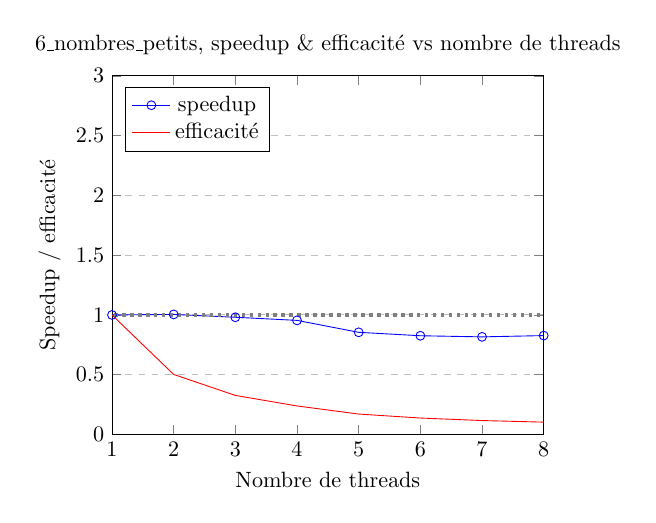
\begin{tikzpicture}[scale=0.8, transform shape]
            \begin{axis}[
                title={6\_nombres\_petits, speedup \& efficacité vs nombre de threads},
                xlabel={Nombre de threads},
                ylabel={Speedup / efficacité},
                xmin=1, xmax=8,
                ymin=0, ymax=3,
                xtick={1,2,3,4,5,6,7,8},
                ytick={0, 0.5, 1, 1.5, 2, 2.5, 3},
                legend pos=north west,
                ymajorgrids=true,
                grid style=dashed,
                ]        
                \addplot[color=blue, mark=o] coordinates {(1, 1)(2, 1.004273321)(3, 0.9805650614)(4, 0.9544884009)(5, 0.8545886935)(6, 0.8258937413)(7, 0.8166147192)(8, 0.8272868789)};        
                \addplot[color=red, mark=] coordinates {(1, 1)(2, 0.5021366604)(3, 0.3268550205)(4, 0.2386221002)(5, 0.1709177387)(6, 0.1376489569)(7, 0.1166592456)(8, 0.1034108599)};
                \addplot[color=gray, dotted, ultra thick] coordinates {(0, 1)(8, 1)};
                \legend{speedup, efficacité}
            \end{axis}
        \end{tikzpicture}
    \end{tabularx}
\end{center}

\newpage

\begin{center}
    \begin{tabularx}{\textwidth}{c c}
        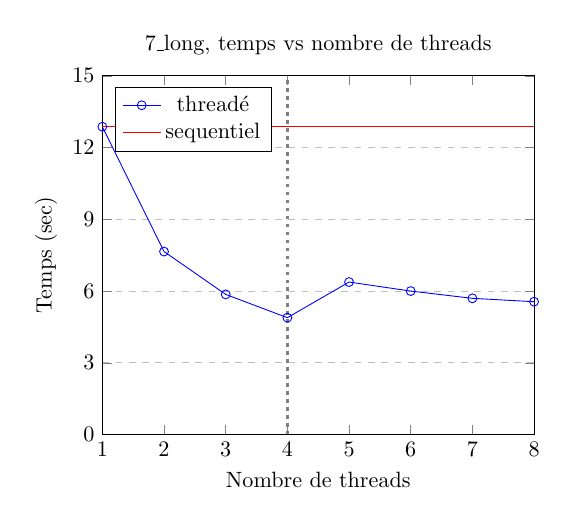
\begin{tikzpicture}[scale=0.8, transform shape]
            \begin{axis}[
                title={7\_long, temps vs nombre de threads},
                xlabel={Nombre de threads},
                ylabel={Temps (sec)},
                xmin=1, xmax=8,
                ymin=0, ymax=15,
                xtick={1,2,3,4,5,6,7,8},
                ytick={0, 3, 6, 9, 12, 15},
                legend pos=north west,
                ymajorgrids=true,
                grid style=dashed,
                ]        
                \addplot[color=blue, mark=o] coordinates {(1, 12.8705)(2, 7.65063)(3, 5.85883)(4, 4.88547)(5,6.37551)(6, 5.99824)(7, 5.69496)(8, 5.55317)};        
                \addplot[color=red, mark=] coordinates {(1, 12.8705)(8, 12.8705)};
                \addplot[color=gray, dotted, ultra thick] coordinates {(4, 0)(4, 15)};
                \legend{threadé, sequentiel}
            \end{axis}
        \end{tikzpicture}
        & 
        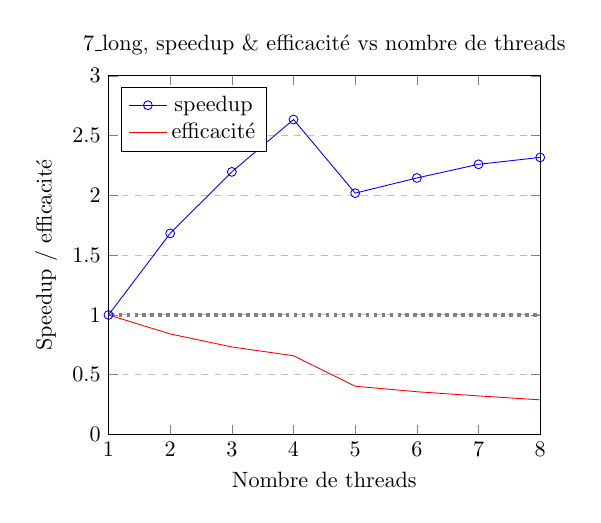
\begin{tikzpicture}[scale=0.8, transform shape]
            \begin{axis}[
                title={7\_long, speedup \& efficacité vs nombre de threads},
                xlabel={Nombre de threads},
                ylabel={Speedup / efficacité},
                xmin=1, xmax=8,
                ymin=0, ymax=3,
                xtick={1,2,3,4,5,6,7,8},
                ytick={0, 0.5, 1, 1.5, 2, 2.5, 3},
                legend pos=north west,
                ymajorgrids=true,
                grid style=dashed,
                ]        
                \addplot[color=blue, mark=o] coordinates {(1, 1)(2, 1.68227976)(3, 2.196769662)(4, 2.634444588)(5, 2.018740462)(6, 2.145712742)(7, 2.259980755)(8, 2.317685214)};        
                \addplot[color=red, mark=] coordinates {(1, 1)(2, 0.84113988)(3, 0.7322565541)(4, 0.6586111469)(5, 0.4037480923)(6, 0.3576187904)(7, 0.3228543936)(8, 0.2897106518)};
                \addplot[color=gray, dotted, ultra thick] coordinates {(0, 1)(8, 1)};
                \legend{speedup, efficacité}
            \end{axis}
        \end{tikzpicture}
        \\
        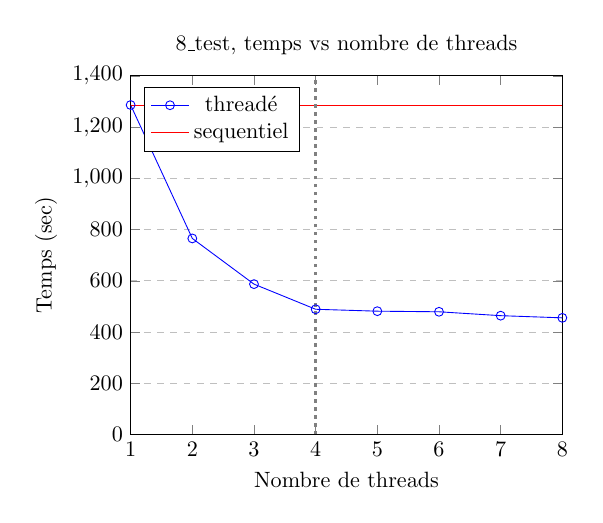
\begin{tikzpicture}[scale=0.8, transform shape]
            \begin{axis}[
                title={8\_test, temps vs nombre de threads},
                xlabel={Nombre de threads},
                ylabel={Temps (sec)},
                xmin=1, xmax=8,
                ymin=0, ymax=1400,
                xtick={1,2,3,4,5,6,7,8},
                ytick={0, 200, 400, 600, 800, 1000, 1200, 1400},
                legend pos=north west,
                ymajorgrids=true,
                grid style=dashed,
                ]        
                \addplot[color=blue, mark=o] coordinates {(1, 1286.07)(2, 765.321)(3, 586.961)(4, 488.817)(5, 481.332)(6, 478.98)(7, 463.821)(8, 455.319)};        
                \addplot[color=red, mark=] coordinates {(1, 1286.07)(8, 1286.07)};
                \addplot[color=gray, dotted, ultra thick] coordinates {(4, 0)(4, 1400)};
                \legend{threadé, sequentiel}
            \end{axis}
        \end{tikzpicture}
        & 
        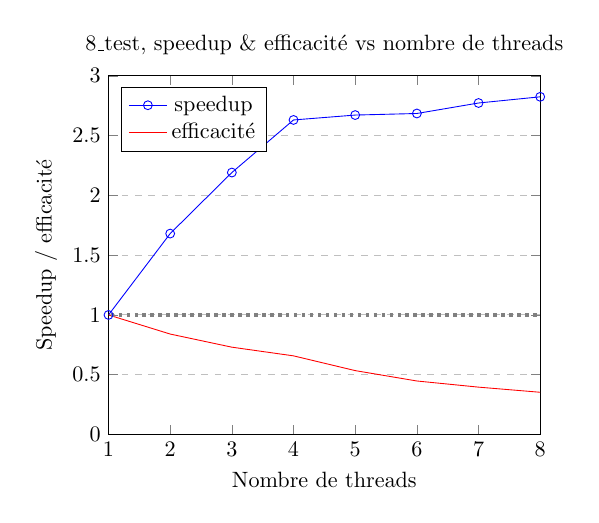
\begin{tikzpicture}[scale=0.8, transform shape]
            \begin{axis}[
                title={8\_test, speedup \& efficacité vs nombre de threads},
                xlabel={Nombre de threads},
                ylabel={Speedup / efficacité},
                xmin=1, xmax=8,
                ymin=0, ymax=3,
                xtick={1,2,3,4,5,6,7,8},
                ytick={0, 0.5, 1, 1.5, 2, 2.5, 3},
                legend pos=north west,
                ymajorgrids=true,
                grid style=dashed,
                ]        
                \addplot[color=blue, mark=o] coordinates {(1, 1)(2, 1.680432132)(3, 2.191065505)(4, 2.630984602)(5, 2.671897983)(6, 2.685018164)(7, 2.772772255)(8, 2.824547186)};        
                \addplot[color=red, mark=] coordinates {(1, 1)(2, 0.8402160662)(3, 0.7303551684)(4, 0.6577461504)(5, 0.5343795966)(6, 0.4475030273)(7, 0.3961103221)(8, 0.3530683982)};
                \addplot[color=gray, dotted, ultra thick] coordinates {(0, 1)(8, 1)};
                \legend{speedup, efficacité}
            \end{axis}
        \end{tikzpicture}
    \end{tabularx}
\end{center}

\section{Analyse}

Avec l'utilisation d'OpenMP, en comparaison avec pthread, nous avons remarqué que le développement
et le debug d'une application multi-threadée est beaucoup plus facile. L'abstraction que propose
OpenMP quant aux contraintes techniques qu'imposent la parallélisation permet d'avoir d'un côté du
code performant (si correctement implémenté évidemment), mais aussi du code lisible, ce qui est plus
compliqué avec pthread. 

Comme expliqué précédemment, nous avons mis en place un algorithme de fusion des intervalles afin de
ne pas dupliquer les calculs sur des nombres contenus dans deux intervalles différents. En
l'appliquant avant le calcul de primalité sur les intervalles, nous avons remarqué que pour certains
fichiers, les intervalles proposés se chevauchent tous, formant alors un seul intervalle final. Étant
donné la structure de notre parallélisation (chaque intervalle est donné à un et un seul thread,
jusqu'à ce que tous les intervalles soient traités), la parallélisation est bornée par le nombre
d'intervalles. De ce fait, les-dits fichiers, (1, 5 et 6) ont des résultats assez peu intéressants
étant donné qu'il sont traités de manière séquentielle. Leurs temps de calcul est presque constant
par rapport au nombre de threads, comportant un peu de bruit. Leurs speedup tendent vers 1 et
l'efficacité décroît rapidement pour tendre vers 0 à un rythme beaucoup plus important que les cas
mieux threadés.

Notre objectif pour ce TP était de minimiser le temps de calcul pour le fichier 8, puisqu'il
représente pour nous l'utilisation la plus propice de la parallélisation de calculs. En effet, les
autres fichiers ayant un temps de traitement suffisamment faible, le temps brut gagné par
parallélisation est presque négligeable. Concernant le fichier 8, le temps de traitement initial est
d'environ 21 minutes, comporte de nombreux intervalles, plus ou moins grands. On remarque que le temps
de calcul passe à 8 minutes pour 4 threads (la machine utilisée possède 4 c\oe urs physiques), donc
presque une division par 3. La qualité de ces résultats est reflétée par le speedup et
l'efficacité. En effet, un speedup de 2.6 (pour 4 threads) indique que la parallélisation répond
bien à ce problème. L'efficacité, valant 0.6 (pour 4 threads) laisse entendre le même résultat
(l'idéal de l'efficacité étant 1). 

Aussi, même si nous avons développé un algorithme pour réduire au plus le temps de traitement du
fichier 8, nous pouvons aussi remarquer que celui-ci donne de bons résultats pour les autres
fichiers possédant plusieurs intervalles ne se recouvrant pas. Par exemple, pour les fichiers 2 et 7, on remarque des résultats
similaires à ceux obtenus pour le fichier 8.

\section{Conclusion}

Notre approche a ses limites, et pourrait être améliorée sur plusieurs points. Nous avons
par ailleurs fait des choix qui sont contestables. Déjà, la mise en place de la fusion des intervalles est
intéressant, cependant cela ne répond pas vraiment au problème demandé. Même si les performances sont
évidemment améliorées, certains fichiers tests sont rendus inutilisables (aussi, cet algorithme de
fusion n'est pas des plus performant, avec une complexité de $O(n)$, $n$ le nombres d'intervalles). Un
deuxième point que nous avons rencontré est notre approche pour la parallélisation. Étant donné le
fonctionnement d'OpenMP, nous n'avons jusque là par trouvé de moyen de paralléliser la boucle
d'itération sur chacun des éléments de chaque intervalle. Paralléliser cette section pourrait donner
des performances bien plus importantes, notamment pour le traitement de peu d'intervalles contenant
beaucoup d'éléments. De plus, nous n'avons pas sélectionné de stratégie d'ordonnancement via OpenMP,
une étude des différentes possibilités ainsi qu'une comparaison des performances de ces derniers
nous aurait sûrement permis d'optimiser un peu plus notre algorithme. Enfin, d'un point de vue plus
technique, le conteneur que nous avons utilisé est \code{std::vector}, dont l'implémentation n'est
pas particulièrement orientée vers la performance (et l'utilisation qu'on en fait n'aide pas).
L'utilisation d'une autre structure, ou même l'implémentation d'un conteneur, serait aussi un moyen
d'améliorer les performances.

Nous avons aussi remarqué que la parallélisation est entre autre limitée par le nombre de threads
que peut gérer le CPU en même temps. Pour améliorer le temps de traitement, l'utilisation d'un
protocole de communication pour distribuer les tâches à travers un réseau d'ordinateurs serait idéal.
L'implémentation de cet algorithme avec MPI permettra sans doute diviser encore plus le temps de
traitement du fichier 8.

\end{document}